\documentclass[12pt]{exam}
\usepackage[
  letterpaper,
  margin=0.3in,
  includehead,    % include the header area in the 0.25in margin
  includefoot     % include the footer area in the 0.25in margin
]{geometry}
\usepackage[shortlabels]{enumitem}
\setlist[enumerate,1]{label=(\alph*)} %makes list alphabetic

\usepackage{physics}

\usepackage{pgfplots} % For sketching graphs
\pgfplotsset{compat=1.18}


\usepackage{caption}

\title{Introduction to Quantum Mechanics - Solution Manual \newline \small{For Griffiths and Schroeter's Third Edition}}

\author{Justin Beltran}
\date{May 2025}

\begin{document}

\maketitle
\firstpagefooter{}{}{By Justin Beltran}
\runningfooter{}{}{By Justin Beltran}
\printanswers

\section{Chapter 1}



\subsection*{Problem 1.1}
For the distribution of ages in the example in Section 1.3.1
\begin{enumerate}[(a)]
    \item  Compute $\expval{j^2}$ and $\expval{j}^2$

    \item Determine $\Delta j$ for each $j$, and use Equation 1.11 to compute the standard deviation.

    \item Use your results in (a) and (b) to check Equation 1.12
\end{enumerate}

\begin{solution}
    \begin{enumerate}[(a)]
        \item There is one person aged 14, one person aged 15, three people aged 16, two people aged 22, two people aged 24, five people aged 25 then 
        $$\expval{j^2} = \sum_j j^2 P(j) = 14^2(\frac{1}{14}) + 15^2(\frac{1}{14}) + 16^2(\frac{3}{14})+ 22^2(\frac{2}{14})+ 24^2(\frac{2}{14})+ 25^2(\frac{5}{14})$$
        $$= \frac{196}{14} + \frac{225}{14}+ \frac{768}{14}+ \frac{968}{14}+ \frac{1152}{14}+ \frac{3125}{14} = \frac{6434}{14} = 459.57$$
        and 
        $$\expval{j}^2 =  \big[\sum_j j^ P(j) = 14(\frac{1}{14}) + 15(\frac{1}{14}) + 16(\frac{3}{14})+ 22(\frac{2}{14})+ 24(\frac{2}{14})+ 25(\frac{5}{14})\big]^2$$
        $$= \big[ \frac{14}{14}+ \frac{15}{14} + \frac{48}{14} + \frac{44}{14} + \frac{48}{14} + \frac{125}{14}\big]^2 = \big[\frac{294}{14}\big]^2 = 21^2 = 441$$

        \item $\expval{j}=21$ then $\Delta j_{14} = 14-21 = -7$, $\Delta j_{15} = 15-21 = -6$, $\Delta j_{16} = 16-21 = -5$,  $\Delta j_{22} = 22-21 = 1$, $\Delta j_{24} = 24-21 = 3$, $\Delta j_{25} = 25-21 = 4$.  Plugging into 1.11 $$\sigma^2 = \expval{(\Delta j)^2}  = (-7)^2(\frac{1}{14}) + (-6)^2(\frac{1}{14}) + (-5)^2(\frac{3}{14})+ 1^2(\frac{2}{14})+ 3^2(\frac{2}{14})+ 4^2(\frac{5}{14})$$ 
        $$
        = 49(\frac{1}{14}) + 36(\frac{1}{14}) + 25(\frac{3}{14})+ (\frac{2}{14})+ 9(\frac{2}{14})+ 16(\frac{5}{14})= \frac{259}{14} = 18.57 \implies\sigma = 4.31$$

        \item Equation 1.12 states $\sigma = \sqrt{\expval{j^2}-\expval{j}^2}$ so plugging in answers from part (a) yields $\sigma =\sqrt{459.57-441} = 18.57$ which is as expected.
    \end{enumerate}
\end{solution}


\subsection*{Problem 1.2}
\begin{enumerate}[(a)]
    \item Find the standard deviation of the distribution in Example 1.2.


    \item What is the probability that a photograph, selected at random, would show a distance $x$ more than one standard deviation away from the average?
\end{enumerate}

\begin{solution}
    \begin{enumerate}[(a)]
        \item Noting that $\expval{x} = \frac{h}{3}$ then $\expval{x}^2 = \frac{h^2}{9}$. Now computing $\expval{x^2} = \int x^2\rho (x)dx$ with $\rho(x) = \frac{1}{2\sqrt{hx}} \implies$
        $$\expval{x^2} = \int^h_0 x^2 \frac{1}{h\sqrt{2x}} dx = \frac{1}{h\sqrt{2}} \int^h_0 x^{1.5}dx =  \frac{1}{h\sqrt{2}} \frac{1}{2.5} x^{2.5} \bigg|^h_0 = \frac{1}{5}h^2$$ plugging it all into $\sigma = \sqrt{\expval{j^2}-\expval{j}^2}$  gives 
        $$\sigma = \sqrt{\frac{h^2}{5}-\frac{h^2}{9}} = \sqrt{\frac{4h^2}{45}} = \frac{2h}{\sqrt{45}}$$

        \item Since the probability of finding the rock is a non-uniform distribution, consider the whole probability subtracted by the probability of being within one standard deviation 
        $$P = 1 - \int^{\expval{x}+\sigma}_{\expval{x}-\sigma} \frac{1}{2\sqrt{hx}}dx = 1-  \frac{1}{2\sqrt{h}}\int^{\expval{x}+\sigma}_{\expval{x}-\sigma} \frac{1}{\sqrt{x}}dx = 1- \frac{1}{2\sqrt{h}}\bigg[2\sqrt{x}\big|^{\expval{x}+\sigma}_{\expval{x}-\sigma}\bigg]$$
        $$=  1- \frac{1}{\sqrt{h}}\bigg[ \sqrt{\expval{x}+\sigma} - \sqrt{\expval{x}-\sigma}\bigg] \text{plugging in} = 1 - \frac{1}{\sqrt{h}}\bigg[ \sqrt{\frac{h}{3}+\frac{2h}{\sqrt{45}}} - \sqrt{\frac{h}{3}-\frac{2h}{\sqrt{45}}}\bigg]$$
        $$ = 1 - 0.795 + 0.188 = 0.393 = 39.3\%$$
    \end{enumerate}
\end{solution}



\subsection*{Problem 1.3}
Consider the \textbf{gaussian} distribution $\rho(x) = Ae^{-\lambda(x-a)^2}$ where $A$, $a$, and $\lambda$ are positive real constants. (The necessary integrals ae inside the back cover.)
\begin{enumerate}[(a)]
    \item Use Equation 1.16 to determine $A$.
    \item Find $\expval{x}, \expval{x^2}$, and $\sigma$.
    \item Sketch the graph of $\rho(x)$
\end{enumerate}

\begin{solution}
    \begin{enumerate}[(a)]
        \item Equation 1.16 states $1 = \int^\infty_{-\infty} \rho(x)dx$ so plugging in 
        $$1 =\int^\infty_{-\infty} Ae^{-\lambda(x-a)^2}dx = A \int^\infty_{-\infty} e^{-\lambda(x-a)^2}dx$$ 
        now let $u = x-a $ then $du = dx$ 
        $$1 =A\int^\infty_{-\infty} e^{-\lambda(u)^2}du = A\frac{1}{\sqrt\lambda}\sqrt{\pi} \implies A = \sqrt{\frac{\lambda}{\pi}}$$

        \item First $$\expval{x} = A \int^\infty_{-\infty} xe^{-\lambda(x-a)^2} dx \text{ let $u = x-a$ then } = A \int^\infty_{-\infty} (u+a)e^{-\lambda(u)^2} du $$
        and let $w = -\lambda u^2$ then $du =\frac{dw}{-\lambda2u}$
        
        $$= A \bigg[\frac{-1}{2\lambda}\int^\infty_{-\infty} e^{w} dw + a\int^\infty_{-\infty} e^{-\lambda u^2} du\bigg] = A\bigg[ \frac{-1}{2\lambda}e^{-\lambda u}\big|^\infty_{-\infty} + a\sqrt{\frac{\pi}{\lambda}} \bigg] = Aa\sqrt{\frac{\pi}{\lambda}} = a$$

        Now computing $\expval{x^2}$  $$\expval{x^2} = A \int^\infty_{-\infty} x^2e^{-\lambda(x-a)^2} dx \text{ let $u = x-a$ then } = A \int^\infty_{-\infty} (u+a)^2e^{-\lambda u^2} du $$
        
        $$\int^\infty_{-\infty} (u^2 + 2au +a^2)e^{-\lambda u^2}du = \int^\infty_{-\infty} u^2 e^{-\lambda u^2}du + 2a\int^\infty_{-\infty}ue^{-\lambda u^2}du + a^2\int^\infty_{-\infty}e^{-\lambda u^2}du$$
        where the right two integrals on the RHS were already computed thus
        $$A\int^\infty_{-\infty} (u+a)^2e^{-\lambda u^2}du  = A\bigg[\int^\infty_{-\infty} u^2 e^{-\lambda u^2}du + 0 + a^2\sqrt{\frac{\pi}{\lambda}} \bigg]$$
        $$ = A\bigg[ 2\sqrt{\pi}2!\big(\frac{1}{2\sqrt{\lambda}}\big)^3 + a^2 \sqrt{\frac{\pi}{\lambda}} \bigg] = A\sqrt{\frac{\pi}{\lambda}} \bigg(\frac{1}{2\lambda} +a^2\bigg) = \frac{1}{2\lambda} +a^2$$

        Lastly calculating $\sigma = \sqrt{\expval{j^2}-\expval{j}^2}$ gives 
        $$\sigma = \sqrt{ \bigg(\frac{1}{2\lambda} +a^2\bigg) - \big(a\big)^2} = \frac{1}{2\lambda}$$

        \item Note that the peak occurs around $x = a$, $\lambda$ controls the stiffness of the peak, and $A$ controls the amplitude. 

        \noindent

        \begin{minipage}[t]{0.45\textwidth}
          \centering
          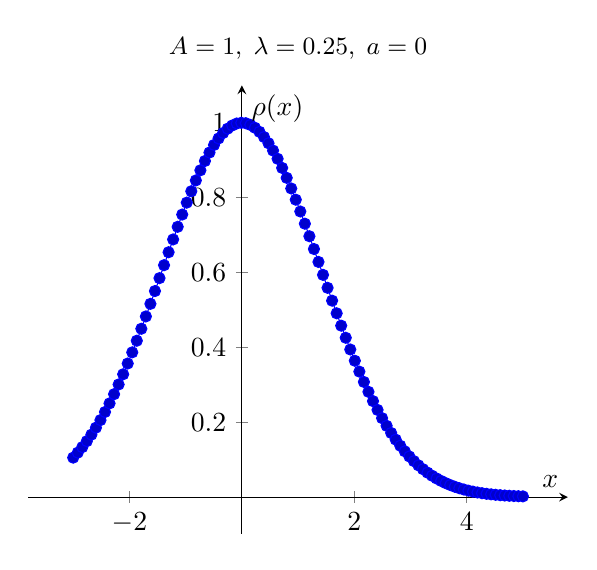
\begin{tikzpicture}
            \begin{axis}[
              domain=-3:5, samples=100,
              xlabel={$x$}, ylabel={$\rho(x)$},
              axis lines=middle, enlargelimits=0.1,
              title={$A=1,\;\lambda=0.25,\;a=0$},  
              title style={font=\small}
            ]
              \addplot {exp(-0.25*(x)^2)};
            \end{axis}
          \end{tikzpicture}
        \end{minipage}\hfill
        \begin{minipage}[t]{0.48\textwidth}
          \centering
          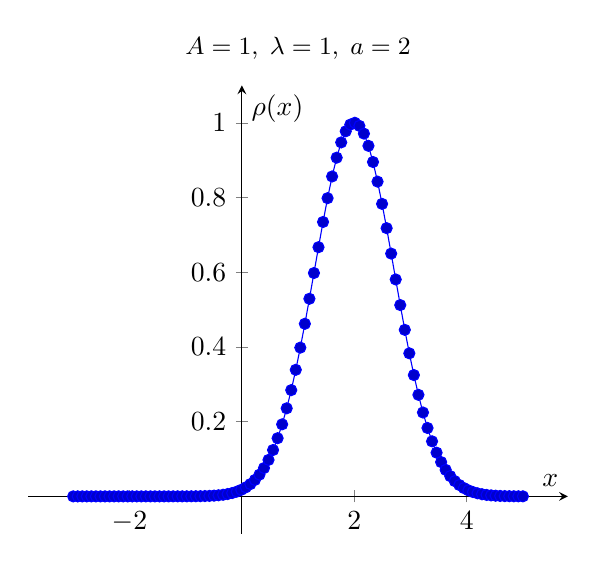
\begin{tikzpicture}
            \begin{axis}[
              domain=-3:5, samples=100,
              xlabel={$x$}, ylabel={$\rho(x)$},
              axis lines=middle, enlargelimits=0.1,
              title={$A=1,\;\lambda=1,\;a=2$},  
              title style={font=\small}
            ]
              \addplot {1*exp(-1*(x-2)^2)};
            \end{axis}
          \end{tikzpicture}
        \end{minipage}

    \end{enumerate}
\end{solution}



\end{document}
